
\chapter{基于压缩后缀数组的序列比对算法}
CSA短读比对算法(CSAA)采用CSA索引参考序列,利用CSA的后向搜索完成匹配过程。CSA的后向搜索是一种精确匹配算法,由于
DNA序列存在变异,以及测序技术有一定的错误率,所以不能简单的使用精确搜索算法。本文提出了两种策略来实现短读比对中的非精确匹配
要求。一是在后向搜索过程中引入了搜索树,使得在搜索过程中可以随时对短读序列进行插入,删除,替换等操作。另一种策略是
采用类似优先队列的数据结构,这一数据结构结合打分机制保证在后向搜索的每一步中都是沿着最优的搜索方向前进,并且采用分支限界
的策略适时淘汰很差的搜索方向。


\subsection{精确匹配}

精确匹配是后向搜索的具体实现。设$T$为长为$n$的参考序列,$P$为测序得到的短读序列中的一个短读,长为$m$。将$P$
映射到$T$上的方法如算法\ref{alg:exac}所示。

\begin{algorithm}
    \caption{精确匹配}
    \label{alg:exac}
    \begin{algorithmic}[1]
        \Require $T,csa,P$
        \Ensure $(l,r)$
        \Function{ExactMatch}{$csa,P$}
        \State $l \gets csa.\alpha(P[m-1])$
        \State $r \gets csa.\alpha(P[m-1])+\beta(P[m-1])-1$
        \For{$i=m-2 \to 0$}
            \If{$l>r$}
                \State \Return $\phi$
            \EndIf
            \State $(l,r) \gets$ \Call{backwardSearch}{$l,r,P[i],csa.\alpha,csa.\beta$}
        \EndFor
        \State \Return $(l,r)$
        \EndFunction
    \end{algorithmic}
\end{algorithm}

算法\ref{alg:exac}采用后向搜索把短读精确匹配到参考序上,返回短读的后缀数组位置$(l,r)$,再利用CSA可以求得$(l,r)$
对应的$T$上的真正位置,完成映射。由于是精确匹配,就只有两种结果,要么匹配上,要么没匹配上,就无需打分机制。这种匹配
方式是完全匹配,但并不适合大多数存在变异和测序误差的短读序列。本文提出的CSAA算法是建立在非精确匹配的基础上的。

\subsection{近似匹配}

由于同一物种之间存在的个体差异以及测序技术存在的误差,Resequencing技术得到的短读序列和该物种的标准参考序列之间
必然存在着不同,这会造成即使同一种基因序列也无法完全比对映射到参考序列上。所以对短读和参考序列之间的比对
仅仅精确比对映射是远远不够的,这会造成大量的短读因为相差一两个碱基而不能映射到参考序列上,而这一两个碱基很可能
是测序误差或者生物个体之间的SNP造成的,不应当认为二者是不能匹配的。所以,采用合适的非精确比对算法是必须的。本文提出的
非精确匹配算法中,支持对短读进行替换(substitude),插入(insert),删除(delete)三种变换操作,通过这三种变换可以保证
变异的或者发生测序错误的短读序列依然能正确匹配到参考序列的合适位置上。

考虑一个给定的长为$m$的短读序列$P$,采用后向搜索,当搜索到第$i+1$个位置时,得到序列$P_{i+1}$的后缀数组位置$(l_{i+1},r_{i+1})$,
依照精确匹配的算法下一步应当在$(l_{i+1},r_{i+1})$的基础上搜索字符$P[i]$,从而得到一个新的后缀数组位置$(l_i,r_i)$。在此,如果我们不
搜索$P[i]$,而是搜索另一个符号$c \neq P[i]$,得到另一个后缀数组位置$(l_{i}^{'},r_{i}^{'})$。接着在$(l_{i}^{'},r_{i}^{'})$基础
上继续搜索$P[0\ldots i-1]$,那么最终得到后缀数组位置$(l_0,r_0)$将不再是序列$P$的一个后缀数组位置了,而是将$P[i]$替换为$c$
后的新字符串的后缀数组位置。称这个新位置为$P$的一个替换近似串的后缀数组位置,计为$(l_0,r_0,m,P(S_i))$,即长为$m$的序列$P$在
$i$位置进行一次替换后可以映射到参考序列的后缀数组位置$(l_0,r_0)$。

图\ref{fig:substitude}给出了把短读序列中的一个符号$T$替换为$A$时的搜索过程,实线为精确匹配的过程,虚线是替换后的搜索过程。

\begin{figure}[htb]
    \centering
    \includegraphics[width=9cm]{substitude.eps}
    \caption{替换操作示例} \label{fig:substitude}
\end{figure}

不同于替换操作,如果在搜索到$P[i]$时,放弃搜索$P[i]$符号,直接在$(l_{i+1},r_{i+1})$的基础上搜索序列$P[0\ldots i-1]$,那么
最终得到的后缀数组位置$(l_0,r_0)$将是$P$删除$P[i]$后的近似串在参考序列上的后缀数组位置,计为$(l_0,r_0,m,P(D_i))$,,即长为$m$
的序列$P$在$i$位置进行一次删除后可以映射到参考序列的后缀数组位置$(l_0,r_0)$。

如图\ref{fig:delete}所示为删除短读序列中的一个符号后的搜索过程。

\begin{figure}[htb]
    \centering
    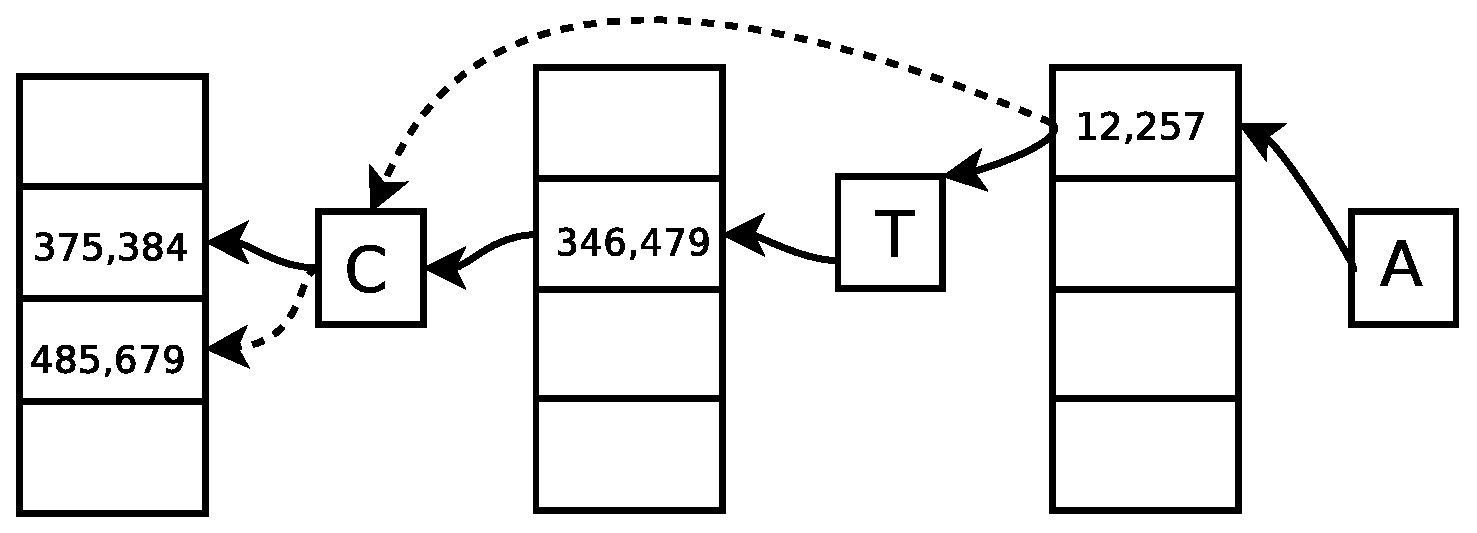
\includegraphics[width=9cm]{delete.eps}
    \caption{删除操作示例} \label{fig:delete}
\end{figure}

对于插入操作,在搜索到$P[i]$时,不直接搜索$P[i]$,而是在$l_{i-1},r_{i-1}$的基础上搜索符号$c$,得到$(l_{i}^{'},r_{i}^{'})$,接着
在此基础上搜索序列$P[0\ldots i]$,最终得到的后缀数组位置$(l_0,r_0)$将是$P$在$i$位置插入符号$c$后的近似序列的后缀数组位置。计为
$(l_0,r_0,m,P(Ii)$,即长为$m$的序列$P$在$i$位置插入一个符号后可以映射到参考序列的后缀数组位置$(l_0,r_0)$。

如图\ref{fig:insert}所示为插入一个符号'A'前后的短读序列中的一个符号后的搜索过程。

\begin{figure}[htb]
    \centering
    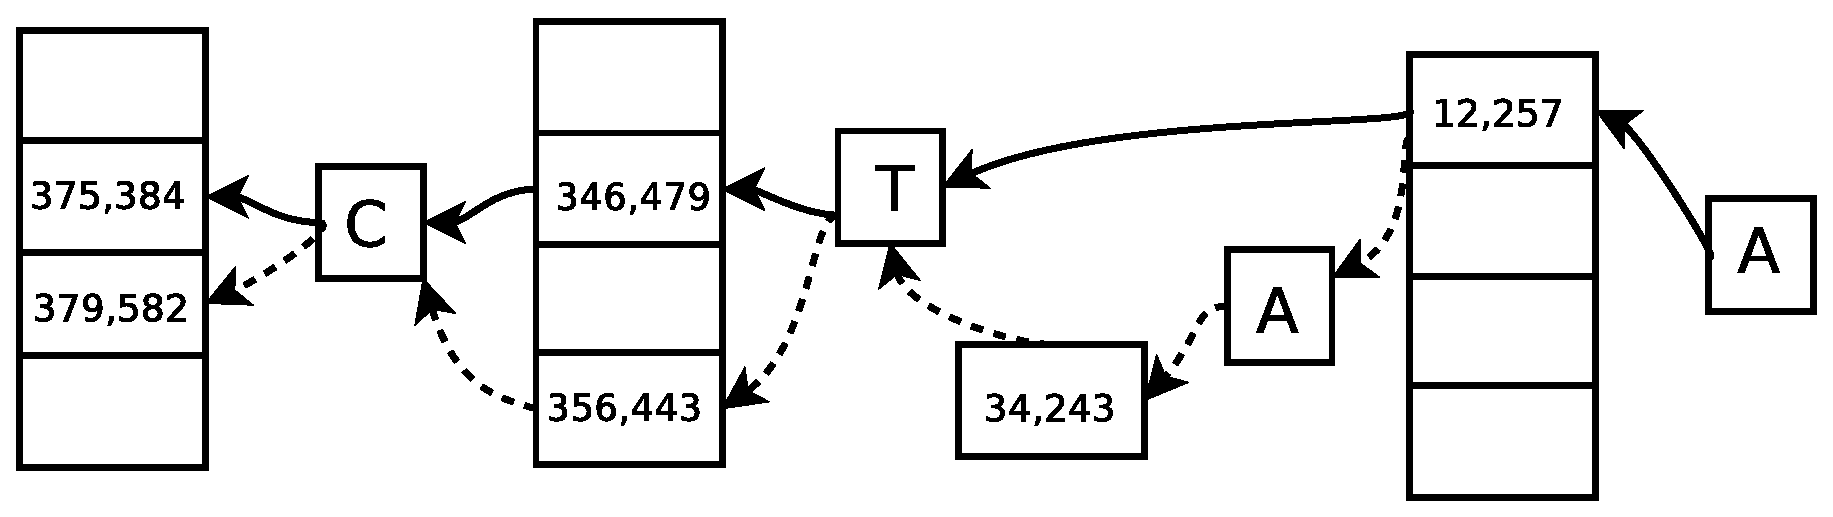
\includegraphics[width=9cm]{insert.eps}
    \caption{插入操作示例} \label{fig:insert}
\end{figure}

\subsubsection{搜索树}

按照上文中描述的用后向搜索实现替换,删除,插入操作的方法,要实现短读序列的近似匹配,在不知道具体的替换,删除以及插入
位置时,需要在每一次后向搜索一个符号时都分别做一次替换,删除,插入操作。而每一次操作实际上都导致了一个新的近似序列的产生,在
未完成整个序列的搜索时,最终哪一个近似序列能够较好的映射到参考序列上依然是未知的,这就要求我们在搜索过程中保留每一个可能的近
似序列。

\begin{figure}[htb]
    \centering
    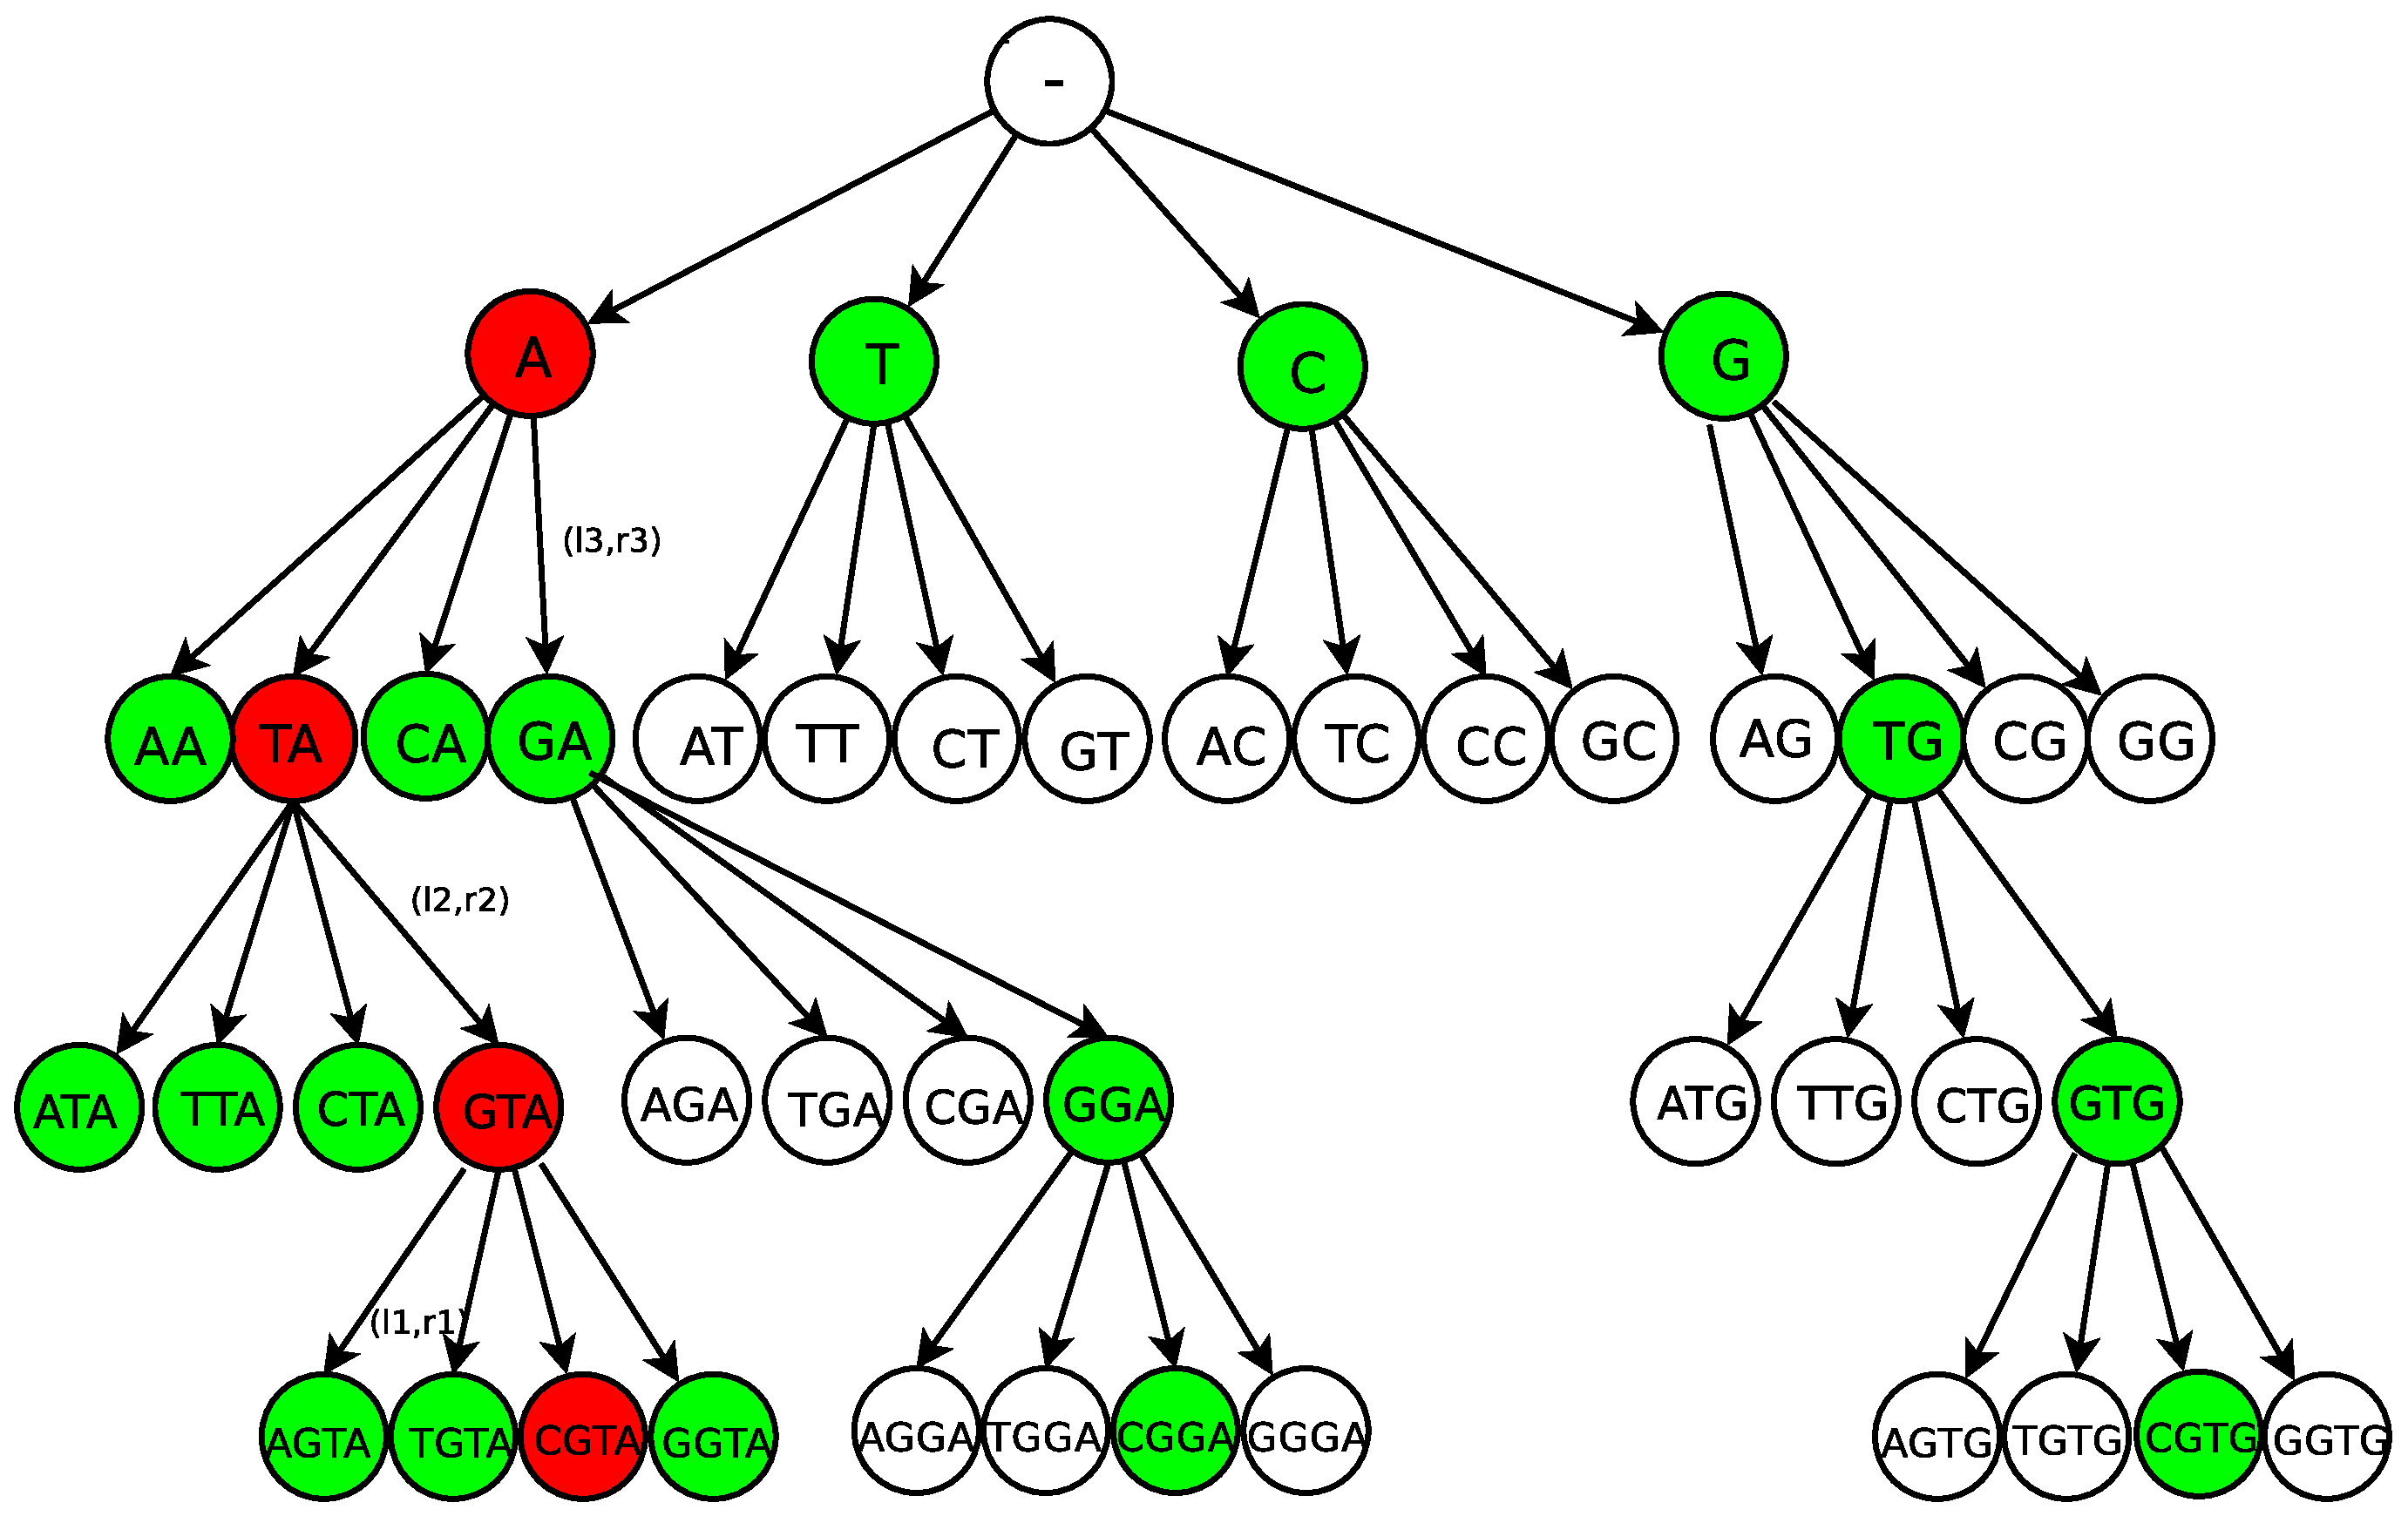
\includegraphics[width=12cm]{searchtree.eps}
    \caption{近似匹配示例} \label{fig:searchtree}
\end{figure}

实际上,每一次的替换,删除或者插入操作导致的新的近似序列可以看作一个树上的遍历过程。如图\ref{fig:searchtree}所示,对于一个长
为4的短读 $P=$``CGTA''的搜索过程,简化起见,省略了删除和插入操作。首先通过CSA查询$P[3]=$`A'在参考序列上的后缀数组位置。接着把
$P[3]=$`A'分别替换为`T',`C',`G',在CSA上查找替换后的后缀数组位置。图中红色路径标志的是到当前搜索深度没有替换操作的近似串,而
绿色标记的则是到当前深度有一次替换操作的近似串,无色的是有两次以上替换操作的近似串搜索路径。可以看到,随着搜索深度的增加,搜索
的方向急剧扩大,加上还有未画出的删除和插入操作,可能的搜索方向会更多。

搜索树的本质是对每一个可能的近似序列都进行搜索,假设一个短读序列的长度为$m$,因为每一个位置都有4种替换,4种插入和1种删除
方法,则总共有$9^m$个近似串。考虑到$m$一般在20到70之间,
如果直接采用搜索树来进行近似匹配,搜索规模会非常大而难以在有效时间内实现。实际上也无需比对所有的近似串,对于某些替换,删除或者插入操作过多的近似串,
应该提前抛弃掉,即采用分支限界法来对搜索树进行剪枝。

\subsubsection{分支限界}

搜索树的规模是指数级增长的,因此必须进行适当的剪枝,抛弃一些没有价值的搜索方向。传统的DNA序列比对中用到了编辑距离,汉明距离
等来度量两个序列的相似度。在此我们也可以使用类似的方法做分支限界,比如采用编辑距离做分支限界。给定一个最大编辑距离$maxdistance$,
当在短读序列$P$上后向搜索进行到第$i$步时,在某个搜索方向上的一个近似序列为$P^{'}$,计算$P$和$P^{'}$之间的编辑距离,若距离大于预先
定义的$maxdistance$,则抛弃这个搜索方向,否则,继续。汉明距离做分支限界的方法和编辑距离方法类似。

采用编辑距离和汉明距离的方法必须对每一个得到的近似序列和短读序列计算距离,这会导致算法效率的降低。实际上,可以采用罚分机制取
代每次都计算编辑距离的开销。在搜索树上向前搜索时,每一次替换,删除或者插入操作都会产生一个新的近似序列,这个序列做了多少次变
换操作是已知的,预定义每一个indel操作的罚分,每一次操作都会对这个近似序列增加相应的罚分,当罚分达到一个预定义的最大罚分
$maxpenalty$
时,即认为这个近似序列已经和短读序列相似度太小,没有必要再搜索下去了。通过这样的罚分机制,可以去除较差的近似序列,而无需
每次都计算编辑距离。

在生物信息学领域,一个indel称为一个空位,对应的罚分称为空位罚分。通常连续的空位的罚分不能简单的做线性增加来处理。
Affine gap penalties是生物信息学领域常用的一种罚分机制,假设有一个连续gap长为$x$,则这个gap的罚分为$-(\rho +\sigma x)$,其中
$\rho >0$,$\sigma$是每一个indel操作的罚分。

除了罚分机制,在论文\cite{li2009fast}中,作者还提出了一种新的高效的分支限界策略,称之为$D(.)$数组。在论文作者实现的短读比对
软件$BWA$中也使用了这一策略来限制搜索空间增长。$D(.)$数组是一个和序列串$P$等长的一个整数数组,$D[i]$取决于序列串$P$的后缀
$P_i$是否是参考序列$T$的一个子串,是的话则增加,不是则归0。具体过程如算法\ref{alg:darray}所示。

\begin{algorithm}
    \caption{计算$D(.)$数组}
    \label{alg:darray}
    \begin{algorithmic}[1]
        \Require $T,csa,P$
        \Ensure $D(.)$
        \Function{CalculateD}{$csa,P$}
            \State $z \gets 0$
            \State $j \gets 0$
            \For{$i \gets 0$ to $|P|-1$}
                \If{$P[j\ldots i]$ is not a substring of $T$}
                    \State $z \gets z+1$
                    \State $j \gets i+1$
                \EndIf
                \State $D[i] \gets z$
            \EndFor
        \EndFunction
    \end{algorithmic}
\end{algorithm}

$D(.)$数组的作用,是结合每一个近似序列的一个辅助值$z$来分支限界的。开始搜索时,序列$P$的$z$值是$D[m-1]$,由算法\ref{alg:darray}
可知,此时的$z$值是$D(.)$数组中最大的值,并且反映了整个序列$P$有多少个连续子串是参考序列的子串。其后在搜索中每进行一次替换,
删除或者插入操作,$z$值都会减小。当搜索到第$i$个位置导致$z<D[i]$时,这个搜索方向将被抛弃。采用$D(.)$数组能够进一步的缩小搜索
空间,提高效率。本文实现的CSAA软件中也把$D(.)$数组作为一个重要的分支限界条件来使用,并取得了较好的结果。

综上所述,本文提出的结合$D(.)$数组和罚分机制做分支限界的搜索树近似匹配算法如下:

\begin{algorithm}[H]
    \caption{近似匹配}
    \label{alg:appro}
    \begin{algorithmic}[1]
        \Require $T,csa,P,maxpenalty$
        \Ensure $\{(l,r)\}$
        \Function{ApproMatch}{$P,i,l,r,z,penalty$}
            \If{$z<D[i]$}
                \State \Return $\phi$
            \EndIf
            \If{$penalty>maxpenalty$}
                \State \Return $\phi$
            \EndIf
            \If{$i<0$}
                \State \Return (l,r)
            \EndIf
            \State $S \gets \phi$
            \State $S \gets S\ \cup$\ \Call{ApproMatch}{$P,i-1,l,r,z-1,penalty+delPenalty$}
            \ForAll{$b \in \{A,T,C,G\}$}
                \State $(l,r)\gets$\Call{backwardSearch}{$l,r,b,csa.\alpha,csa.\beta$}
                \If{$l\leq r$}
                \State $S \gets S\ \cup\ $ \Call{ApproMatch}{$P,i,l,r,z-1,penalty+insPenalty$}
                    \If {$b=P[i]$}
                    \State $S \gets S\ \cup$\ \Call{ApproMatch}{$P,i-1,l,r,z,penalty$}
                    \Else
                    \State $S \gets S\ \cup$\ \Call{ApproMatch}{$P,i-1,l,r,z-1,penalty+subPenalty$}
                    \EndIf
                \EndIf
            \EndFor
            \State \Return $S$
        \EndFunction
    \end{algorithmic}
\end{algorithm}

算法\ref{alg:appro}是本文提出的CSAA算法的核心,采用两种分支限界策略,减小搜索空间,能够完成替换,插入和删除三种变换操作,
实现近似搜索。算法\ref{alg:appro}同时使用了后向搜索算法\ref{alg:backwardsearch}。该算法只是一个理论形式,具体实现中必须做一些修改。


